\begin{tikzfigure}
    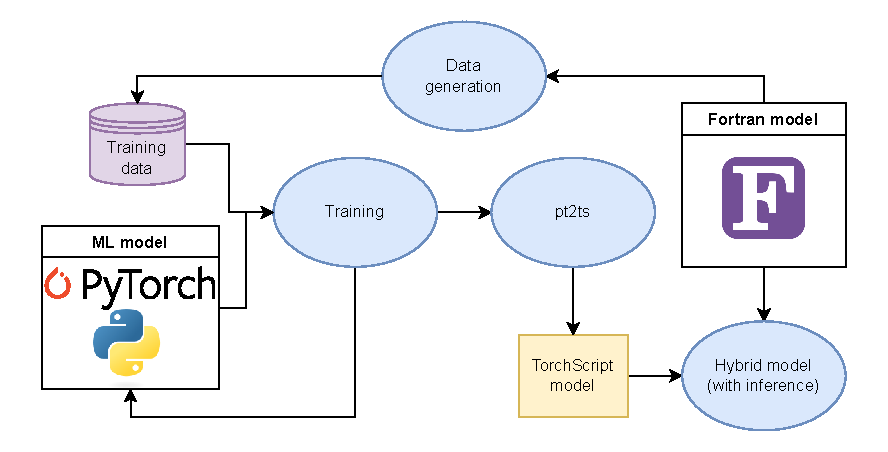
\includegraphics[width=0.44\textwidth]{figures/offline-training-diagram.pdf}
\end{tikzfigure}
\begin{itemize}
    \setlength{\itemsep}{0pt}
    \item \textbf{Design the ML model in PyTorch} with PyTorch \faPython~API
    \item \textbf{Dataset generation} for the ML model training via Fortran-based model runs
    \item \textbf{Train} the PyTorch model on generated data, optimizing for the specific predictive tasks
    \item \textbf{pt2ts} Convert trained  models (\texttt{.pt}) to TorchScript (\texttt{.ts})
    \item \textbf{Hybrid model} Integrate the TorchScript model with\\ Fortran code using FTorch, enabling inference during runs
\end{itemize}
